\documentclass[12pt]{article}
\usepackage[margin=1in]{geometry}
\usepackage{graphicx}
\usepackage{booktabs}
\usepackage{amsmath}
\usepackage{amssymb}
\usepackage{float}
\usepackage{caption}
\usepackage{setspace}
\usepackage[most]{tcolorbox}
\captionsetup{font=small, labelfont=bf, skip=6pt}
\onehalfspacing
\graphicspath{{figures/}}

\newtcolorbox{explain}{%
  colback=black!3,
  colframe=black!25,
  boxrule=0.5pt,
  arc=1pt,
  left=8pt,
  right=8pt,
  top=5pt,
  bottom=5pt,
  before skip=6pt,
  after skip=12pt,
  fontupper=\normalsize
}

\title{Forecast Significance Tests\\[0.2em]
\large Diebold--Mariano on the test window}
\author{Volatility forecasting project}
\date{1 October 2026}

\begin{document}
\maketitle

\noindent
Pairwise Diebold--Mariano tests for HAR, the standalone LSTM, and the HAR+LSTM hybrid
on the test window (\(n=999\)).
Runner: \texttt{reports/run\_significance.py}.
This note does not change the main project report or the split-compare report.

\section{How to read the plots}
\begin{itemize}
  \item Loss differentials: \(d_t=L_t^{A}-L_t^{B}\). Negative means \(A\) is better.
  \item DM statistic: mean of \(d_t\) over a Newey--West HAC standard error
    (lag \(\lfloor n^{1/3}\rfloor\)).
  \item Dashed lines at \(\pm 1.96\): rough 5\% two-sided cutoff.
  \item Green bars: \(p<0.05\). Grey bars: not significant.
\end{itemize}
\begin{explain}
LSTM vs HAR and HAR vs LSTM are the same test with opposite sign:
\(d_t^{\mathrm{HAR}-\mathrm{LSTM}}=-d_t^{\mathrm{LSTM}-\mathrm{HAR}}\).
The DM statistic flips sign, the \(p\)-value is identical, and ``who is better'' swaps.
They are shown both ways only for readability.
\end{explain}

\section{Mean test loss}
\begin{figure}[H]
\centering
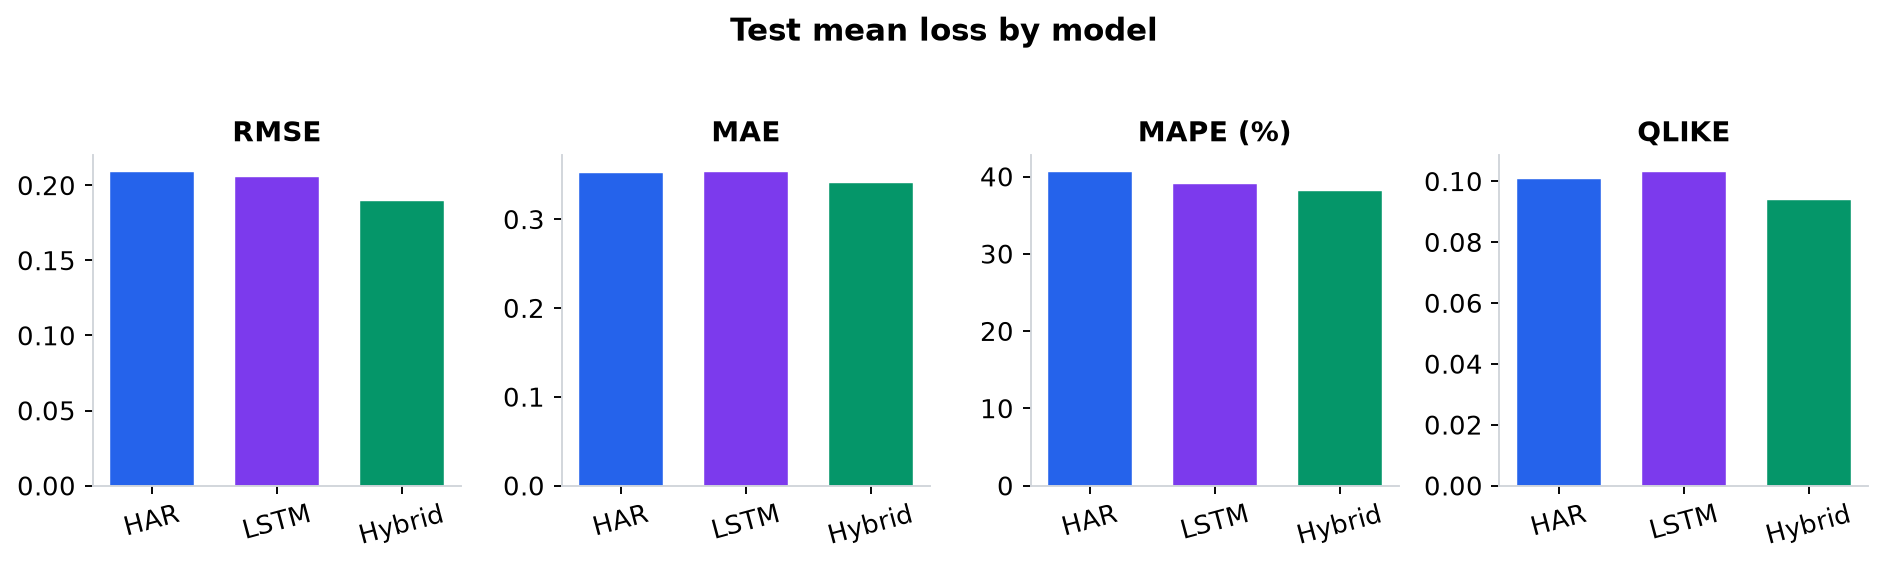
\includegraphics[width=\textwidth]{significance_mean_loss.png}
\caption{Average test loss for HAR, LSTM, and Hybrid.
RMSE/MAE panels use log-RV losses; MAPE is in percent; QLIKE is on RV.}
\end{figure}
\begin{explain}
Hybrid is lowest on every panel. LSTM is close to HAR on RMSE/MAE/QLIKE and lower on MAPE.
\end{explain}

\section{DM statistics}
\begin{figure}[H]
\centering
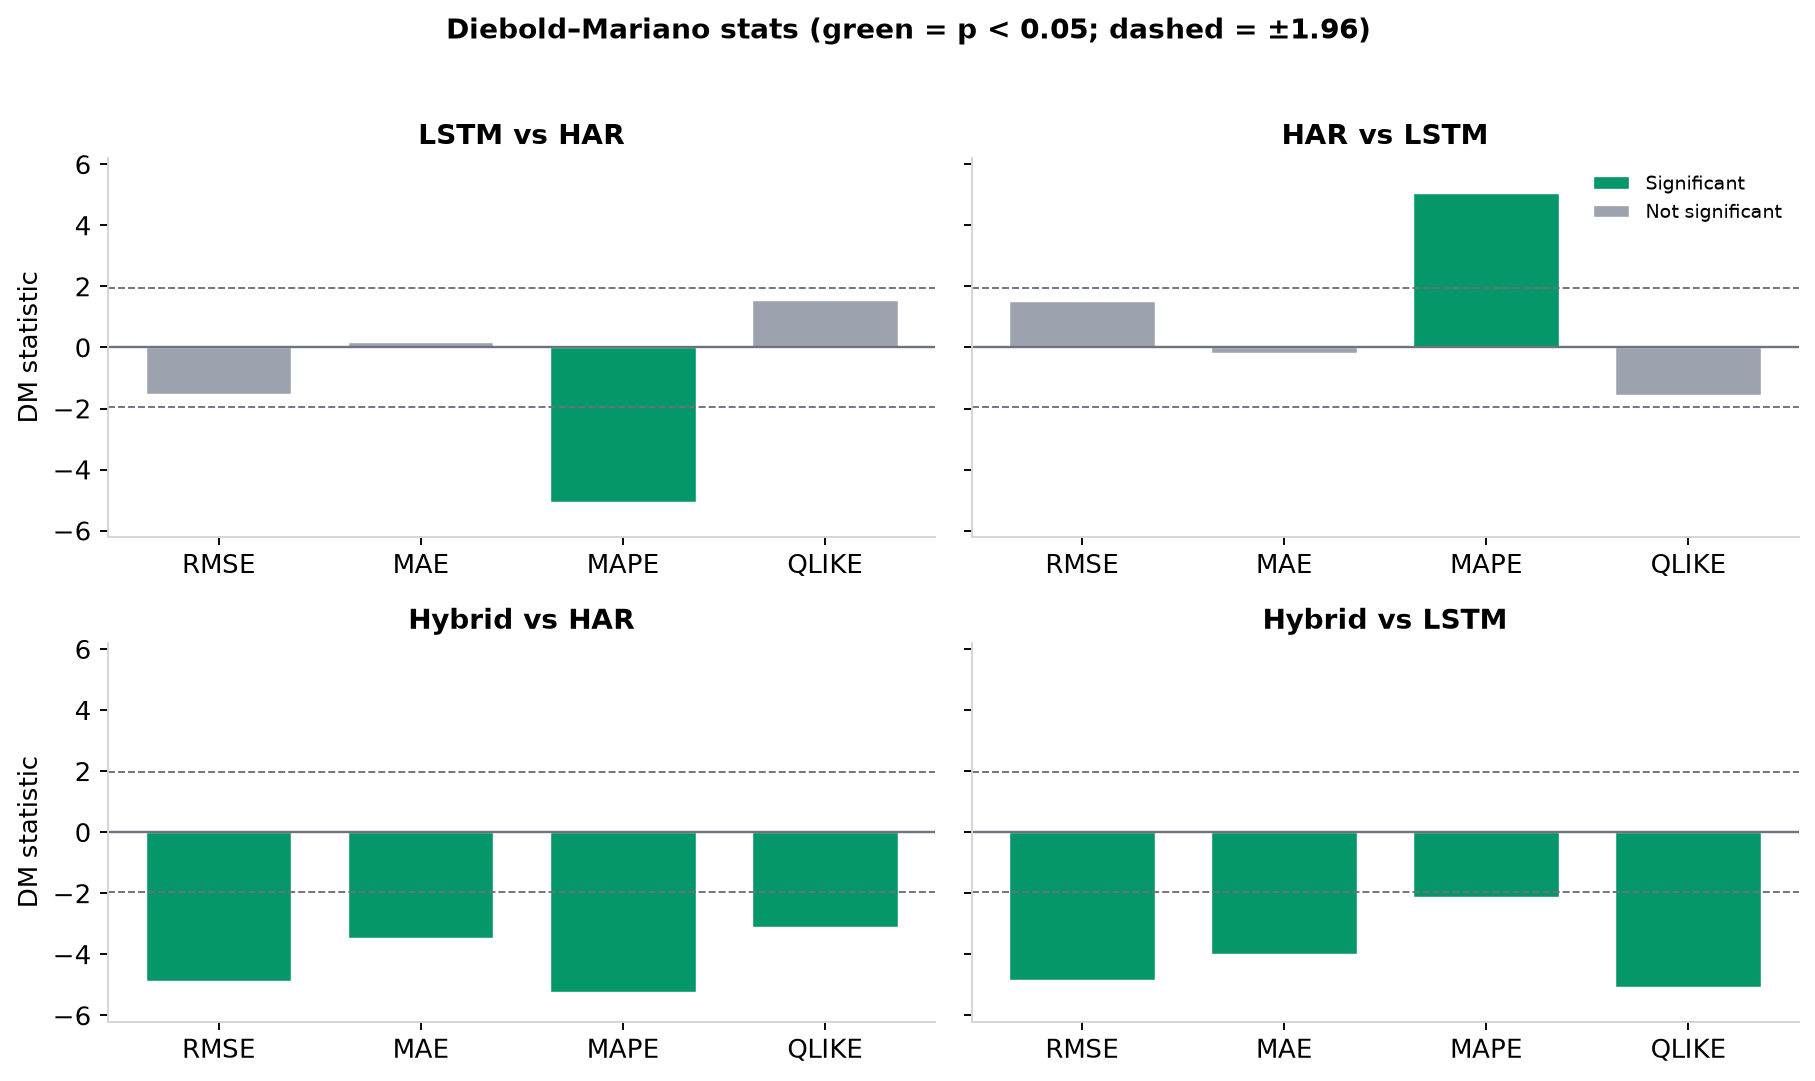
\includegraphics[width=0.98\textwidth]{significance_dm_bars.png}
\caption{DM statistics by pair and loss. Negative bars favor the first model in the title.
Green means significant at 5\%. Top row: LSTM vs HAR and its mirror HAR vs LSTM.}
\end{figure}
\begin{explain}
LSTM vs HAR: only MAPE clears the significance line. RMSE, MAE, and QLIKE stay inside
\(\pm 1.96\). HAR vs LSTM is the vertical flip of that panel (same \(p\)-values).
Hybrid vs HAR and Hybrid vs LSTM: all four losses are significant.
\end{explain}

\section{Cumulative squared-error gap}
\begin{figure}[H]
\centering
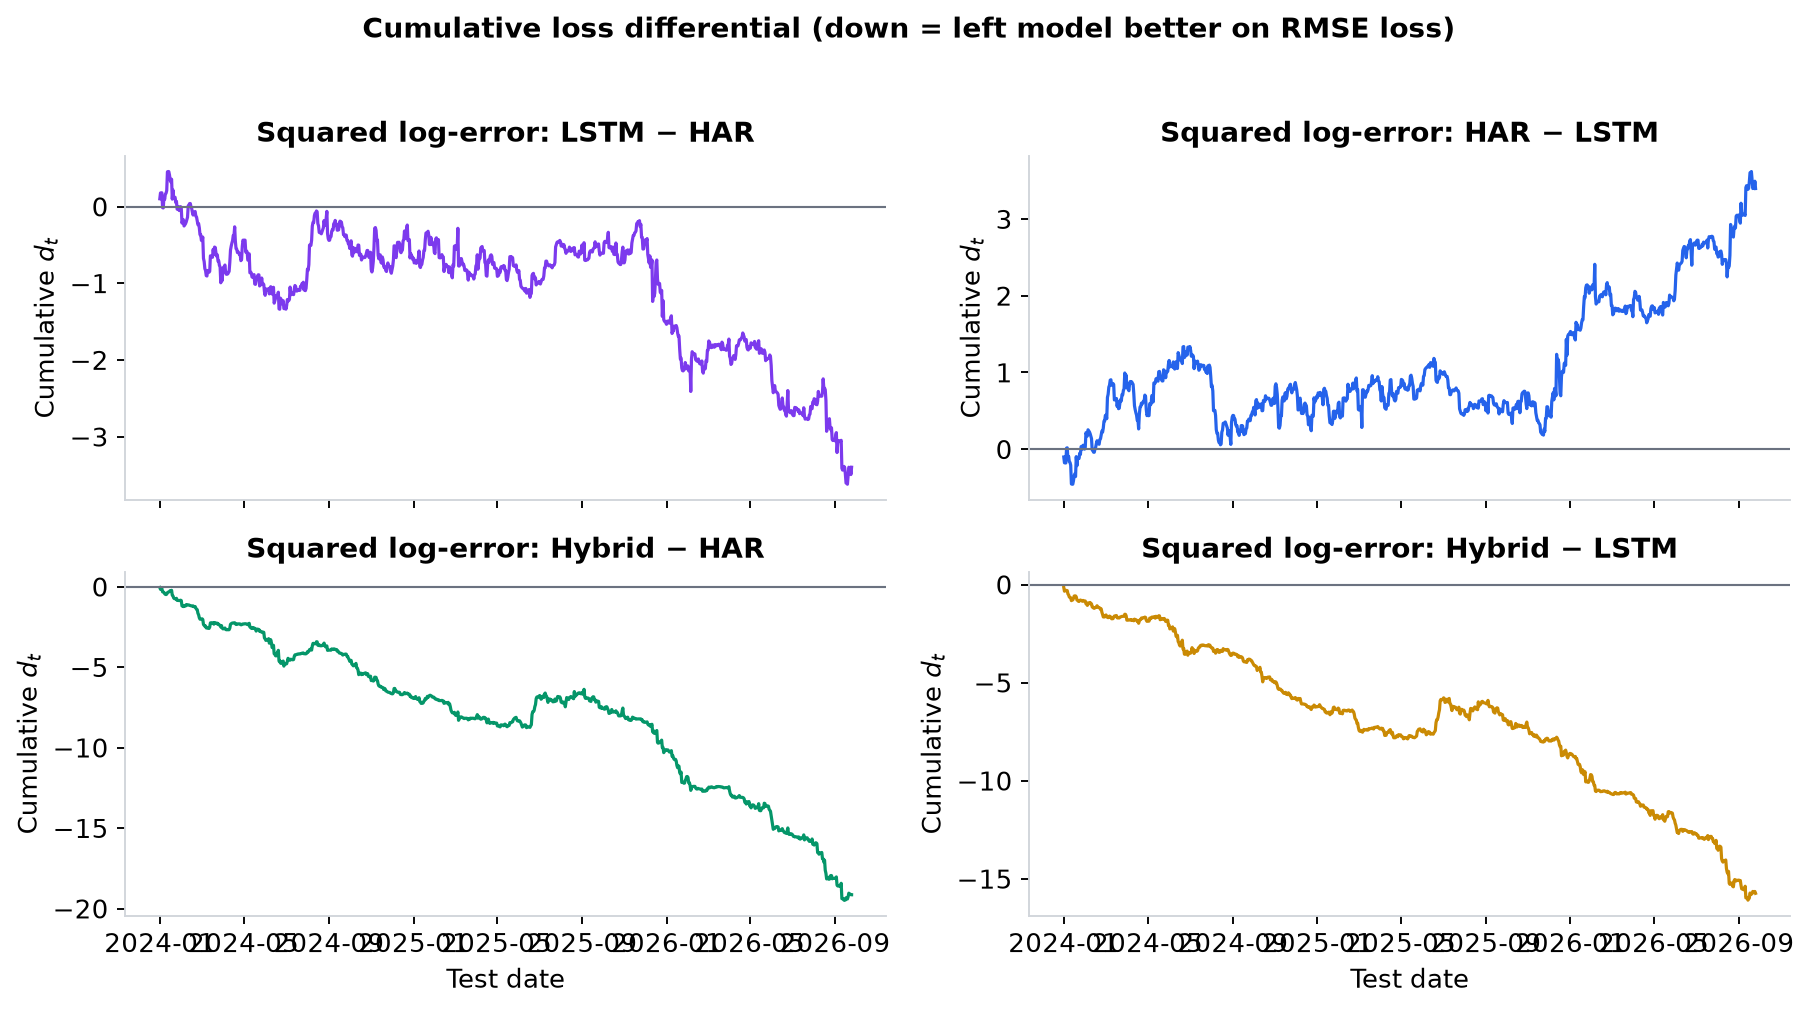
\includegraphics[width=\textwidth]{significance_cumdiff.png}
\caption{Running sum of squared log-error differentials on the test path.
A path that drifts down means the left-hand model is accumulating lower RMSE loss.
HAR $-$ LSTM is the pointwise flip of LSTM $-$ HAR.}
\end{figure}
\begin{explain}
LSTM vs HAR wanders near zero: the RMSE edge does not build a clean lead.
HAR vs LSTM is that path flipped. Hybrid vs HAR and Hybrid vs LSTM drift down through the test sample.
\end{explain}

\section{Numbers (compact)}
\begin{table}[H]
\centering
\begin{tabular}{llrrl}
\toprule
Pair & Loss & DM & \(p\) & Better \\
\midrule
LSTM vs HAR & RMSE & $-1.53$ & $0.127$ & n.s. \\
LSTM vs HAR & MAE & $+0.19$ & $0.847$ & n.s. \\
LSTM vs HAR & MAPE & $-5.07$ & $<10^{-6}$ & LSTM \\
LSTM vs HAR & QLIKE & $+1.57$ & $0.117$ & n.s. \\
\midrule
HAR vs LSTM & RMSE & $+1.53$ & $0.127$ & n.s. \\
HAR vs LSTM & MAE & $-0.19$ & $0.847$ & n.s. \\
HAR vs LSTM & MAPE & $+5.07$ & $<10^{-6}$ & LSTM \\
HAR vs LSTM & QLIKE & $-1.57$ & $0.117$ & n.s. \\
\midrule
Hybrid vs HAR & RMSE & $-4.89$ & $<10^{-5}$ & Hybrid \\
Hybrid vs HAR & MAE & $-3.48$ & $0.0005$ & Hybrid \\
Hybrid vs HAR & MAPE & $-5.24$ & $<10^{-6}$ & Hybrid \\
Hybrid vs HAR & QLIKE & $-3.10$ & $0.0019$ & Hybrid \\
\midrule
Hybrid vs LSTM & RMSE & $-4.84$ & $<10^{-5}$ & Hybrid \\
Hybrid vs LSTM & MAE & $-3.98$ & $<10^{-4}$ & Hybrid \\
Hybrid vs LSTM & MAPE & $-2.11$ & $0.035$ & Hybrid \\
Hybrid vs LSTM & QLIKE & $-5.07$ & $<10^{-6}$ & Hybrid \\
\bottomrule
\end{tabular}
\caption{Two-sided DM tests. ``n.s.'' = not significant at 5\%.
HAR vs LSTM mirrors LSTM vs HAR (sign flip, same \(p\)).}
\end{table}

\end{document}
